\documentclass[12pt]{article}
\usepackage[margin=1in]{geometry} 
\usepackage{amsmath}
\usepackage{amssymb}
\usepackage{siunitx}
\usepackage{float}
\usepackage{tikz}
\def\checkmark{\tikz\fill[scale=0.4](0,.35) -- (.25,0) -- (1,.7) -- (.25,.15) -- cycle;} 
\usepackage{url}
\usepackage[siunitx,american,RPvoltages]{circuitikz}
\ctikzset{capacitors/scale=0.7}
\ctikzset{diodes/scale=0.7}
\usepackage{tabularx}
\newcolumntype{C}{>{\centering\arraybackslash}X}
\renewcommand\tabularxcolumn[1]{m{#1}}% for vertical centering text in X column
\usepackage{tabu}
\usepackage[spanish,es-tabla,activeacute]{babel}
\usepackage{babelbib}
\usepackage{booktabs}
\usepackage{pgfplots}
\usepackage{hyperref}
\hypersetup{colorlinks = true,
            linkcolor = black,
            urlcolor  = blue,
            citecolor = blue,
            anchorcolor = blue}
\usepgfplotslibrary{units, fillbetween} 
\pgfplotsset{compat=1.16}
\usepackage{bm}
\usetikzlibrary{arrows, arrows.meta, shapes, 3d, perspective, positioning,mindmap,trees,backgrounds}
\renewcommand{\sin}{\sen} %change from sin to sen
\usepackage{bohr}
\setbohr{distribution-method = quantum,insert-missing = true}
\usepackage{elements}
\usepackage{verbatim}
\usepackage[edges]{forest}
\usepackage{etoolbox}
\usepackage{schemata}
\usepackage{appendix}
\usepackage{listings}

\definecolor{color_mate}{RGB}{255,255,128}
\definecolor{color_plas}{RGB}{255,128,255}
\definecolor{color_text}{RGB}{128,255,255}
\definecolor{color_petr}{RGB}{255,192,192}
\definecolor{color_made}{RGB}{192,255,192}
\definecolor{color_meta}{RGB}{192,192,255}
\newcommand\diagram[2]{\schema{\schemabox{#1}}{\schemabox{#2}}}

\definecolor{codegreen}{rgb}{0,0.6,0}
\definecolor{codegray}{rgb}{0.5,0.5,0.5}
\definecolor{codepurple}{rgb}{0.58,0,0.82}
\definecolor{backcolour}{rgb}{0.95,0.95,0.92}

\lstdefinestyle{mystyle}{
    backgroundcolor=\color{backcolour},   
    commentstyle=\color{codegreen},
    keywordstyle=\color{magenta},
    numberstyle=\tiny\color{codegray},
    stringstyle=\color{codepurple},
    basicstyle=\ttfamily\footnotesize,
    breakatwhitespace=false,         
    breaklines=true,                 
    captionpos=b,                    
    keepspaces=true,                 
    numbers=left,                    
    numbersep=5pt,                  
    showspaces=false,                
    showstringspaces=false,
    showtabs=false,                  
    tabsize=2
}

\lstset{style=mystyle}
\usepackage{lastpage}
\usepackage{fancyhdr}
\pagestyle{fancy}
\setlength{\headheight}{42pt}
\setlength{\parindent}{0cm}
 
\begin{document}
\sisetup{unit-math-rm=\mathrm,math-rm=\mathrm} % change sinitx font
\sisetup{output-decimal-marker = {,}}
\lhead{Ingeniería en Mantenimiento Industrial \\ Escuela de Ingeniería Electromecánica \\ Tecnológico de Costa Rica} 
\rhead{Electricidad I \\ Tarea \#2  \\ Entrega: Semana 8} 
\cfoot{\thepage\ de \pageref{LastPage}}
Antes de continuar leyendo este documento, conteste las siguientes preguntas:
\begin{itemize}
    \item ¿Que es un modelo de un sistema? 
    \item ¿Que es un experimento?   
    \item ¿Que es una simulación? ¿Es toda simulación un experimento?
\end{itemize}

Definiciones y ecuaciones para celdas y baterías:
\begin{itemize}
    \item Celda electroquímica recargable: es un dispositivo capaz de convertir energía química en energía electrica y viceversa. 
    \item Batería: es la interconexión de dos o mas celdas electroquímicas.
    \item Capacidad nominal [$Q$]: es la cantidad de carga que una celda o batería puede entregar en amperios-hora (\si{\ampere\hour})
    \item Eficiencia de Coulumb [$\eta$]: es la eficiencia con la que se transfiere la carga a una batería, tipicamente se asume que $\eta = 1$ durante la descarga y que $\eta < 1$ durante la carga. 
    \item SOC [$z(t)$]: \emph{state of charge}, estado de carga de una celda o batería, para una celda o batería descargada $z(t) = 0$, mientras que para una celda o batería cargada $z(t) = 1$. El estado de carga se puede relacionar con la corriente por medio de la siguiente ecuación:
    \begin{equation*}
        z(t) = z(t_0) - \dfrac{1}{Q}\int_{t_0}^t \eta i(\tau) d\tau
    \end{equation*}
    \item Tasa C: \emph{C Rate}, es una medida relativa de la corriente en una celda o batería usando como base la capacidad, por ejemplo si una celda tiene una capacidad de \SI{3}{\ampere\hour} y se descarga a corriente constante con una taza de $0.5$C entonces la corriente debe ser $i=0.5\cdot 3 = \SI{1.5}{\ampere}$
    \item OCV: \emph{open circuit voltage}, voltaje de circuito abierto es el voltaje que la celda o batería tendría si se desconecta de la carga y se deja descansar hasta que el valor del voltaje sea constante. 
    \item CC: se refiere a un proceso de carga o descarga que se realiza con corriente constante
    \item CV: se refiere a un proceso de carga o descarga que se realiza con voltaje constante
\end{itemize}

Existe gran diversidad de modelos para celdas electroquímicas de iones de Litio (Li-Ion), el modelo mas sencillo es una simple fuente independiente que representa el voltaje en los terminales de la celda, los modelos mas complejos incluyen la resistencia interna del electrolito y las interfaces entre el electrolito y el electrodo, el efecto de la eficiencia de Coulomb y los efectos de la difusión de los iones.\\[8pt]
En la Figura \ref{fig:Rint} se muestra un modelo sencillo para un celda electroquímica, este tipo de modelo se conoce como \emph{Rint}

\begin{figure}[H]
    \centering
    \begin{circuitikz}
        \draw 
        (0,0)
            to[cV, l=OCV$(z)$]
        (0,3)
            to[R, l=$R_0$,i=$i(t)$,-o]
        (3,3)
            to[open,v^=$v(t)$]
        (3,0)
            to[short,o-]
        (0,0)
        ;
    \end{circuitikz}
    \caption{Circuito Rint}
    \label{fig:Rint}
\end{figure}

\textbf{Instrucciones}
\begin{enumerate}
    \item Se le facilita un archivo de valores separados por comas (csv) llamado ``OCV(z).csv'' que incluye los valores del voltaje de circuito abierto para los estados de carga comprendidos entre $0.2$ y $1$. Estos valores fueron obtenidos por medio de pruebas de laboratorio realizadas en el \href{https://www.tec.ac.cr/unidades/laboratorio-delta}{DeltaLab} a una celda tipo NCR18650B de Panasonic (Ver Figura \ref{fig:18650}). Puede descargarlo \href{https://estudianteccr-my.sharepoint.com/:x:/g/personal/prof_juan_rojas_estudiantec_cr/EaWEaD9eY35Clh4iO77cZ5YBe0Tf2joTGQHzCdW8IVIatA?e=91HoDB}{acá}
    \item Asuma que $Q = \SI{3250}{\milli\ampere\hour}$, $z(t_0) = 0.25$, $R_0 = \SI{85}{\milli\ohm}$, $\eta = 1$ para los procesos de descarga y $\eta = 0.98$ para los procesos de carga. Considere un proceso de carga/descarga en el que la celda se carga en CC a $1$C hasta que $v(t)=\SI{4.2}{\volt}$ y luego de eso se carga en CV a \SI{4.2}{\volt} hasta que la corriente es sea igual a \SI{300}{\milli\ampere}, luego de esto la celda se descarga a $1$C hasta que $v(t)=\SI{3.2}{\volt}$.
    \item Usando Python cree un \emph{script} llamado ``calculos'' que le permita realizar lo siguiente:
    \begin{itemize}
        \item leer los datos del archivo ``OCV(z).csv'', guardarlos en una o varias matrices y crear una función que permita ingresar cualquier valor de $z$ y recibir el valor correspondiente de OCV($z$) usando interpolación lineal (la interpolación lineal debe ser implementada por el estudiante desde cero) 
        \item programar el proceso de carga-descarga descrito en el punto 2 usando los conceptos y leyes básicas vistos en el curso, aproximando la integral que describe $z(t)$ por medio de una discretización con un intervalo de \SI{0.25}{\second}, esto es: 
        \begin{equation*}
            z[k+1] = z[k] - \dfrac{\eta \Delta t}{Q}i[k]
        \end{equation*}
        donde $\Delta t$ es el intervalo de integración discreta, en este caso \SI{0.25/3600}{\hour}; $z[k]$ e $i[k]$ son los valores actuales del SOC y la corriente respectivamente; y $z[k+1]$ es el valor siguiente del SOC
        \item generar una gráfica que en las abscisas tenga los valores del tiempo $t$ y en las ordenadas tenga el valor del voltaje $v(t)$
        \item generar una gráfica que en las abscisas tenga los valores del tiempo $t$ y en las ordenadas tenga el valor de la corriente $i(t)$. 
        \item generar una gráfica que en las abscisas tenga los valores del tiempo $t$ y en las ordenadas tenga el valor del SOC $z(t)$.
        \item imprimir en la terminal el valor del SOC inicial, SOC al final de la carga, SOC al final de la descarga, la capacidad cargada y la capacidad descargada.
    \end{itemize}
    \item Realice un informe de su tarea llamado ``Informe\_t2.tex'' usando \LaTeX. Incluya todos los cálculos y las gráficas solicitadas y algún texto complementario que permita entender la solución realizada. Un machote se puede encontrar \href{https://www.overleaf.com/read/phnwtckqwqwc}{acá}
    \item Comprima todo en un solo archivo .zip y suba al TecDigital. Cualquier entrega tardía se califica con base en 70. 
\end{enumerate}

\begin{figure}[H]
    \centering
    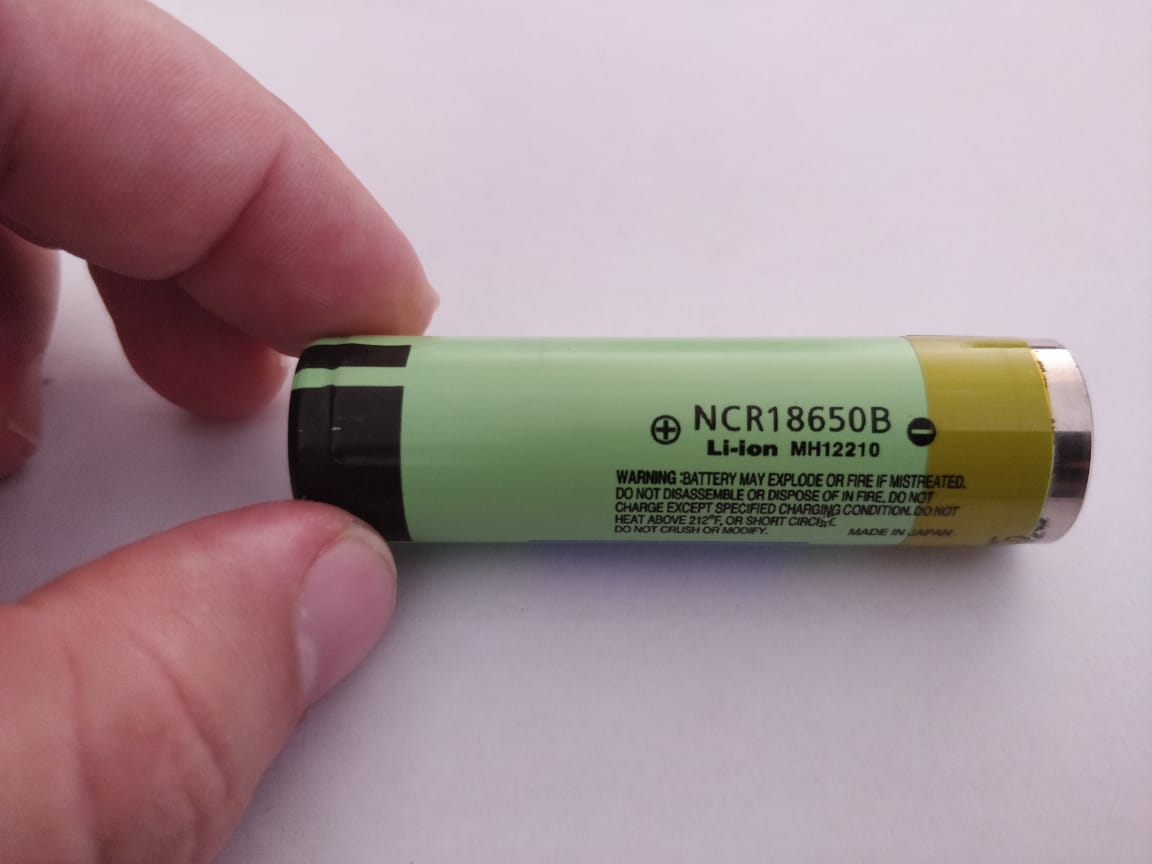
\includegraphics[width=0.6\linewidth]{fig/NCR18650.jpeg}
    \caption{Celda NCR18650B de Panasonic}
    \label{fig:18650}
\end{figure}

% \bibliographystyle{IEEEtran}
% \bibliography{ref_tareas}

\end{document}